%-*- coding: UTF-8 -*-
% 论文总结.tex
% 2020年7月第二周
\documentclass[UTF8]{ctexart}
\usepackage{graphicx}
\usepackage{float}
\usepackage{amsmath}
\usepackage{geometry}
\geometry{a4paper,centering,scale=0.8}
\usepackage[format=hang,font=small,textfont=it]{caption}
\usepackage[nottoc]{tocbibind}
\usepackage{url}
\usepackage{listings}
\usepackage{booktabs}
\usepackage{xcolor}     %高亮使用的颜色
\definecolor{commentcolor}{RGB}{85,139,78}
\definecolor{stringcolor}{RGB}{206,145,108}
\definecolor{keywordcolor}{RGB}{34,34,250}
\definecolor{backcolor}{RGB}{220,220,220}

\lstset{
 columns=fixed,       
 numbers=left,                                        % 在左侧显示行号
 numberstyle=\tiny\color{gray},                       % 设定行号格式
 frame=none,                                          % 不显示背景边框
 backgroundcolor=\color[RGB]{245,245,244},            % 设定背景颜色
 keywordstyle=\color[RGB]{40,40,255},                 % 设定关键字颜色
 numberstyle=\footnotesize\color{darkgray},           
 commentstyle=\it\color[RGB]{0,96,96},                % 设置代码注释的格式
 stringstyle=\rmfamily\slshape\color[RGB]{128,0,0},   % 设置字符串格式
 showstringspaces=false,                              % 不显示字符串中的空格
 language=c++,                                        % 设置语言
}

\newenvironment{myquote}
{\begin{quote}\kaishu\zihao{-5}}
{\end{quote}}

\newcommand\degree{^\circ}

\title{\heiti \section{总结}\label{sec:diyijie}}
\title{\heiti Real_Time Multistep Attack Prediction Based on Hidden Markov Models}
\author{\kaishu 海华}
\date{\today}

\bibliographystyle{plain}

\newtheorem{thm}{定理}

\begin{document}
    \section{背景介绍}\label{sec:diyijie}
  	数据访问策略的错误配置已经成为导致安全事件发生的主要原因。当用户抱怨自己被拒绝访问时,系统管理员需要立即解决用户的问题,就可能存在过多授权的问题。
	\begin{figure}[ht]
        \centering
        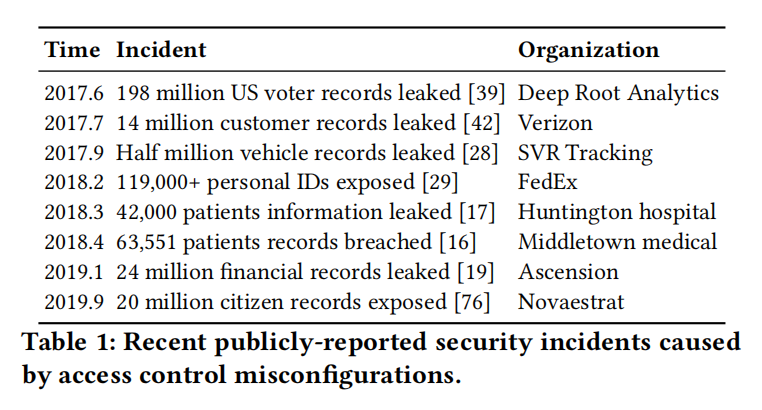
\includegraphics[scale=0.5]{picture/001.png}
        \caption{框架}
        \label{fig:001}
    \end{figure}
    \clearpage
	\section{基于现有访问控制机制观察}\label{sec:dierjie}

	本文创新:
	\begin{itemize}
	\item[1] 不同的软件系统实现了不同的访问控制模型,即使是相同的访问控制模型,策略配置的语法和格式也可能存在不同。
	\item[2] 不同的访问控制日志都有统一的格式而且比较容易解析。都可以表示为四元组<S,O,A,R>,其中S表示subject,O表示object,A表示action,R表示result(result分为allow和deny)。所有的访问控制策略都可以使用if-then语句表示。
基于以上几点,作者想到了用决策树来处理。但是传统的决策树无法解决带时间序列的问题、策略更新的编码问题。
	\end{itemize}
	\clearpage
	\section{P-DIFF模型}\label{sec:disanjie}
	主要解决的三个问题:
	\begin{itemize}
	\item[1] 怎么去维系策略策略改变历史?-Time-Changing Decision Tree (TCDT)
	\item[2] 如何从访问日志中推断访问策略?-a decision-tree-based learning algorithm
	\item[3] 如何管理改变之后的策略?
	\end{itemize}
	\begin{figure}[ht]
        \centering
        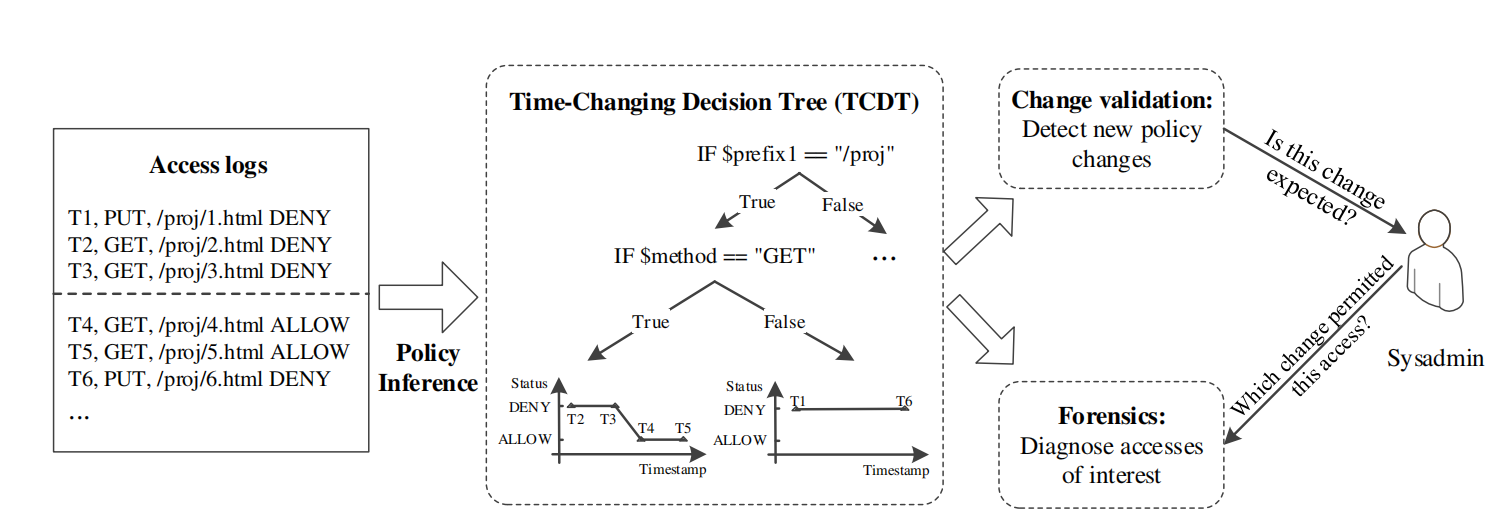
\includegraphics[scale=0.5]{picture/002.png}
        \caption{P-DIFF模型}
        \label{fig:001}
    \end{figure}
	\clearpage
	\section{DT和TCDT}\label{sec:disijie}
	\begin{itemize}
	\item[1] decision tree:节点分为两种:内部节点和叶子节点。内部节点表示(属性名 属性值)。subject、object和action都可以是属性。结果是(r,pr),r表示结果,pr表示结果的概率。
	\item[2] time-changing decision tree:结果表示为: 
	\begin{equation}\label{eq:mi}
    \begin{aligned}
    &T=((\tau_1,r_1),(\tau_n,r_n),...,(\tau_n,r_n))
    \end{aligned}
    \end{equation}
	引入了时间序列的概念。
	\end{itemize}
	\clearpage
	\section{一种基于决策树的学习算法}\label{sec:diwujie}
	特征抽取:
	\begin{figure}[ht]
        \centering
        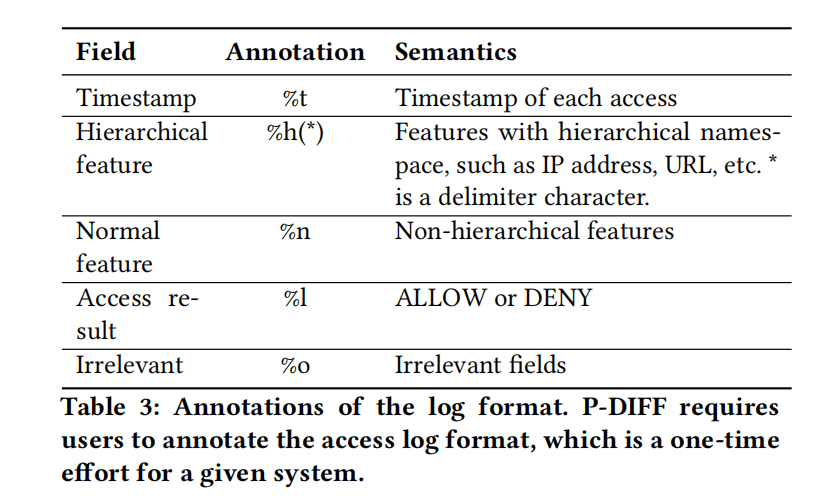
\includegraphics[scale=0.5]{picture/003.png}
        \caption{特征提取}
        \label{fig:003}
    \end{figure}
    算法步骤:
	\begin{figure}[ht]
        \centering
        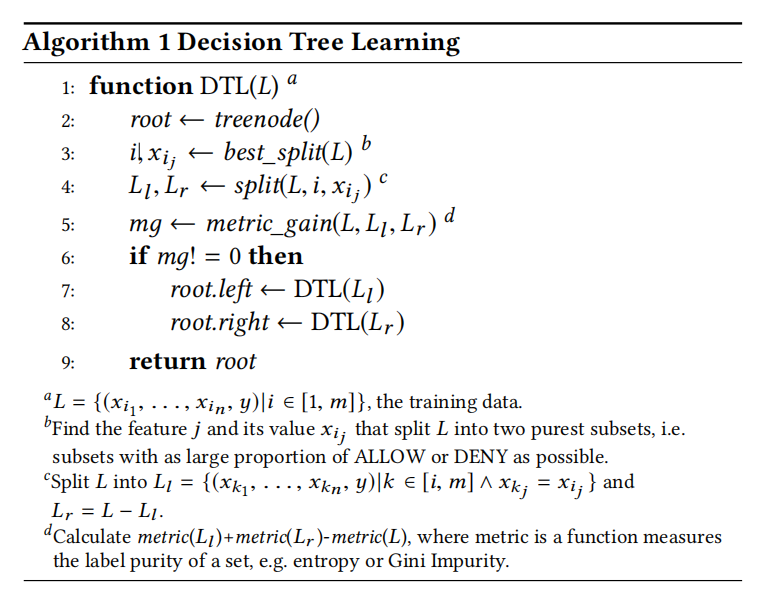
\includegraphics[scale=0.5]{picture/004.png}
        \caption{算法步骤}
        \label{fig:004}
    \end{figure}
	\clearpage
	\section{策略改变管理}\label{sec:diliujie}
	\begin{figure}[ht]
        \centering
        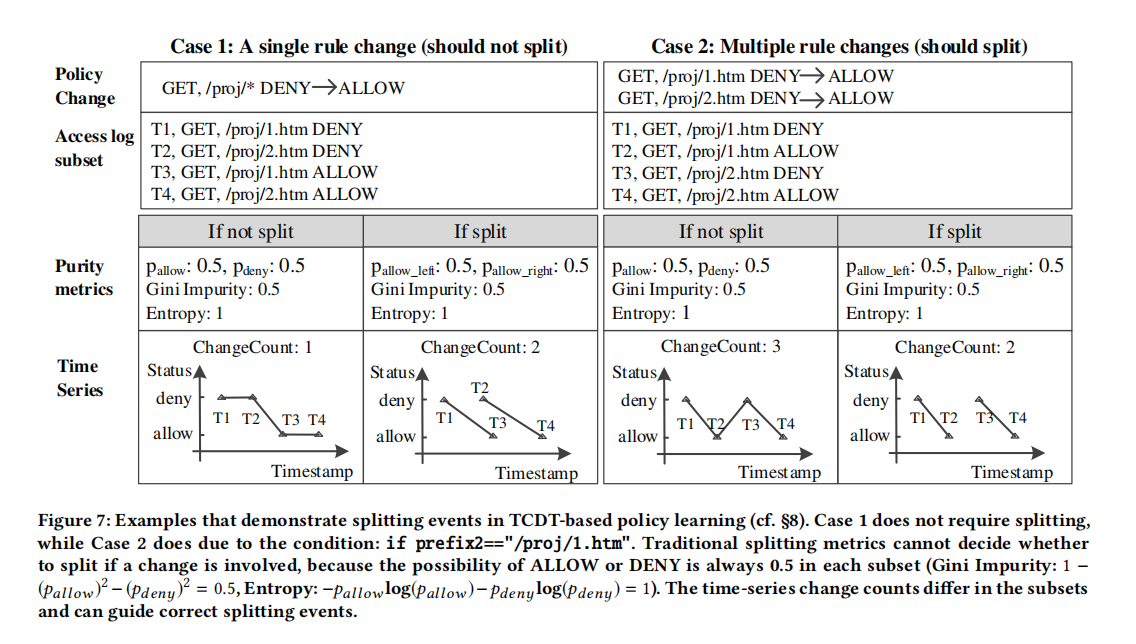
\includegraphics[scale=0.5]{picture/005.png}
        \caption{算法步骤}
        \label{fig:005}
    \end{figure}
	\clearpage
	\section{优化}\label{sec:diqijie}
	优化点:1)循环中只计算deny的值   2)离散卷积的方法
	\begin{figure}[ht]
        \centering
        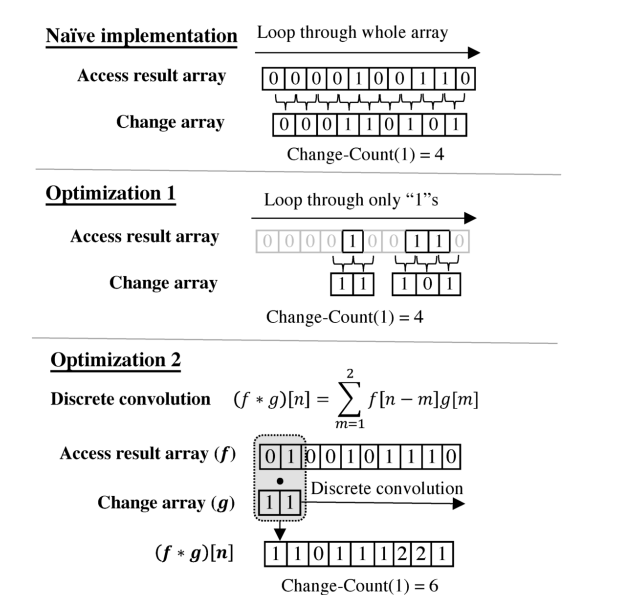
\includegraphics[scale=0.5]{picture/006.png}
        \caption{算法步骤}
        \label{fig:006}
    \end{figure}
	\clearpage
	\section{实验评估}\label{sec:dibajie}
	TCDT:准确率:0.997  召回率:0.92	F-score:0.94

	spark-dl:准确率:0.83  召回率:0.86   F-score:0.80
	\begin{figure}[ht]
        \centering
        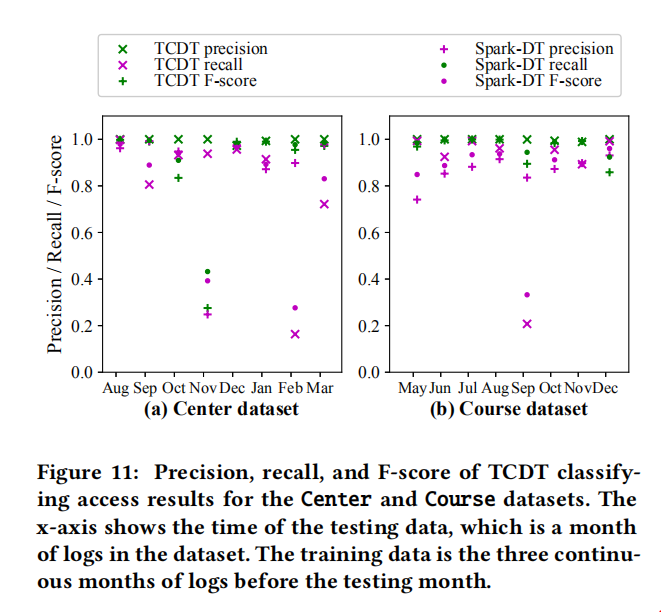
\includegraphics[scale=0.5]{picture/007.png}
        \caption{算法步骤}
        \label{fig:007}
    \end{figure}
	\clearpage
	\bibliography{test}
\end{document}

